% Default mode is landscape, which is what we want, however dvips and
% a0poster do not quite do the right thing, so we end up with text in
% landscape style (wide and short) down a portrait page (narrow and
% long). Printing this onto the a0 printer chops the right hand edge.
% However, 'psnup' can save the day, reorienting the text so that the
% poster prints lengthways down an a0 portrait bounding box.
%
% 'psnup -w85cm -h119cm -f poster_from_dvips.ps poster_in_landscape.ps'

\documentclass[a0]{a0poster}
\pagenumbering{gobble}
% You might find the 'draft' option to a0 poster useful if you have
% lots of graphics, because they can take some time to process and
% display. (\documentclass[a0,draft]{a0poster})

\pagestyle{empty}
\renewcommand{\d}{\mathrm{d}}
\newcommand{\sgn}[1]{\mathop{\mathrm{sgn}}#1}
\newcommand{\bu}{\mathbf{u}}
\newcommand{\bx}{\mathbf{x}}
\newcommand{\br}{\mathbf{r}}
\newcommand{\ds}{\mathrm{d}s}
\newcommand{\ie}{\textit{i.e.}}
\setcounter{secnumdepth}{0}
\newcommand{\comment}[1]{}

% The textpos package is necessary to position textblocks at arbitary 
% places on the page.
\usepackage[absolute]{textpos}
% Graphics to include graphics. Times is nice on posters, but you
% might want to switch it off and go for CMR fonts.
\usepackage[final]{graphics}
\usepackage{wrapfig,helvet}
\usepackage{amsmath}

% For using urls
\usepackage{hyperref}

% For citations
\usepackage{cite}

% These colours are tried and tested for titles and headers. Don't
% over use color!
\usepackage{color}
\definecolor{DarkBlue}{rgb}{0.1,0.1,0.5}
\definecolor{Red}{rgb}{0.9,0.0,0.1}
\definecolor{headingcol}{rgb}{0.5,0.7,1}
%\definecolor{boxcol}{rgb}{0.3,0.8,0.1}

% see documentation for a0poster class for the size options here
\let\Textsize\normalsize
\def\Head#1{
  \noindent\hbox to \hsize{\hfil{\LARGE\color{DarkBlue}\sf #1}}\bigskip}
\def\LHead#1{\noindent{\LARGE\color{DarkBlue}\sf #1}\bigskip}
\def\Subhead#1{\noindent{\large\color{DarkBlue}\sf #1}\bigskip}
\def\Title#1{\noindent{\VeryHuge\color{Red}\bf\sf #1}}

\TPGrid[40mm,40mm]{23}{12}  % 3 cols of width 7 plus 2 gaps width 1

\parindent=0pt
\parskip=0.5\baselineskip

\makeatletter                         %Needed to include code in main file
\renewcommand\@maketitle{             %
\null			              %Sets position marker
{
\color{headingcol}\sffamily\VERYHuge  %Set title font and colour
\@title \par}%
\vskip 0.6em%
{
\color{white}\sffamily\LARGE	      %Set author font and colour
\lineskip .5em%
\begin{tabular}[t]{l}%
\@author
\end{tabular}\par}%
\vskip 1cm
\par
}
\makeatother

\title{Addressing cold start in music recommendation}

\author{Wiktor Grajkowski and Ioannis Gakos\\ University College London}

\begin{document}
  %----------------------------------------------------------------------%
  %           Title bar: across all 21 columns                           %
  %----------------------------------------------------------------------%
  \begin{textblock}{23}(0,0)
  \vspace*{-48mm}\hspace*{-42mm}%
  
\includegraphics{ucl_bar_black.eps}
  \begin{minipage}{1191mm}		%Minipage for title contents
  \vspace{-20cm}
  \maketitle
  \end{minipage}
  \end{textblock}

  %%%%%%%%%%%%%%%%%% Will need to shift all other content down a bit %%%%%

  %----------------------------------------------------------------------%
  %           First column.                                              %
  %----------------------------------------------------------------------%
  \begin{textblock}{7}(0,2.4)
    \Head{Introduction}
    \sf % Selects sans serif family: part of the UCL corporate image!
    Our goal is to build a music recommendation system using a Convolutional
    Neural Network (CNN). CNNs have been widely used in applications such as
    image recognition and recommendation systems. The promiment shift of the
    music industry towards the Web, has made music recommendation a rather
    relevant problem whose solution could radically improve users' experience.
    However, in the absence of usage data, existing methods such as
    collaborative filtering fall short in taking effective decisions for new
    and unpopular content. [1]
    \\ \\
    The design is based on recent work of A\"{a}ron van den Oord et al. on
    music recommendation [1] using deep CNNs and on Dieleman's post on the
    implementation details of such CNN built during his internship at
    Spotify. Our main objective is to build a system that addresses the cold
    start problem for both new users and music content. Users give a single
    preferred track as input, based on which a shuffled playist with relevant
    music content is generated. Newly imported music content is classified
    based on its frequency spectrum and the already existing ground truth data,
    without using any usage related feedback. In order to train the CNN model,
    the MagnaTagATune open dataset will be used, which contains 26,000 user
    annotated audio samples.

    \bigskip
    \hrule
  \end{textblock}

  \begin{textblock}{7}(0,6.0)
    \Head{The Problem}
    \sf 
    Traditional content recommendation systems rely on user usage data to make
    decisions. Behavior patterns between users, are used by collaborative
    filtering methods to make recommendations about various types of content.
    However, collaborative filtering suffers from the cold start problem.

    Latent factor vectors are compact representations of the users'
    preferences correlated with other characteristics of the items. Predicting
    these vectors for new music content based only on metadata such as the
    artist's name is often impossible. Using audio content to predict latent
    factor vectors can bridge the semantic gap between the characteristics of
    an audio track and the users' preferences. A\"{a}ron van den Oord et al.
    converted existing usage data, present in the MagnaTagATune dataset, to the
    latent vector space using Weighted Matrix Factorization and trained a CNN
    using these vectors to minimize the Mean Squeared Error of the predicted
    latent vectors of audio samples. Visualization of their qualititave 
    evaluation is depicted in Figure 1.
    
    \hspace*{1cm}
    \begin{center}
      \begin{figure}
      \centering
      \rotatebox{0}{\scalebox{1}{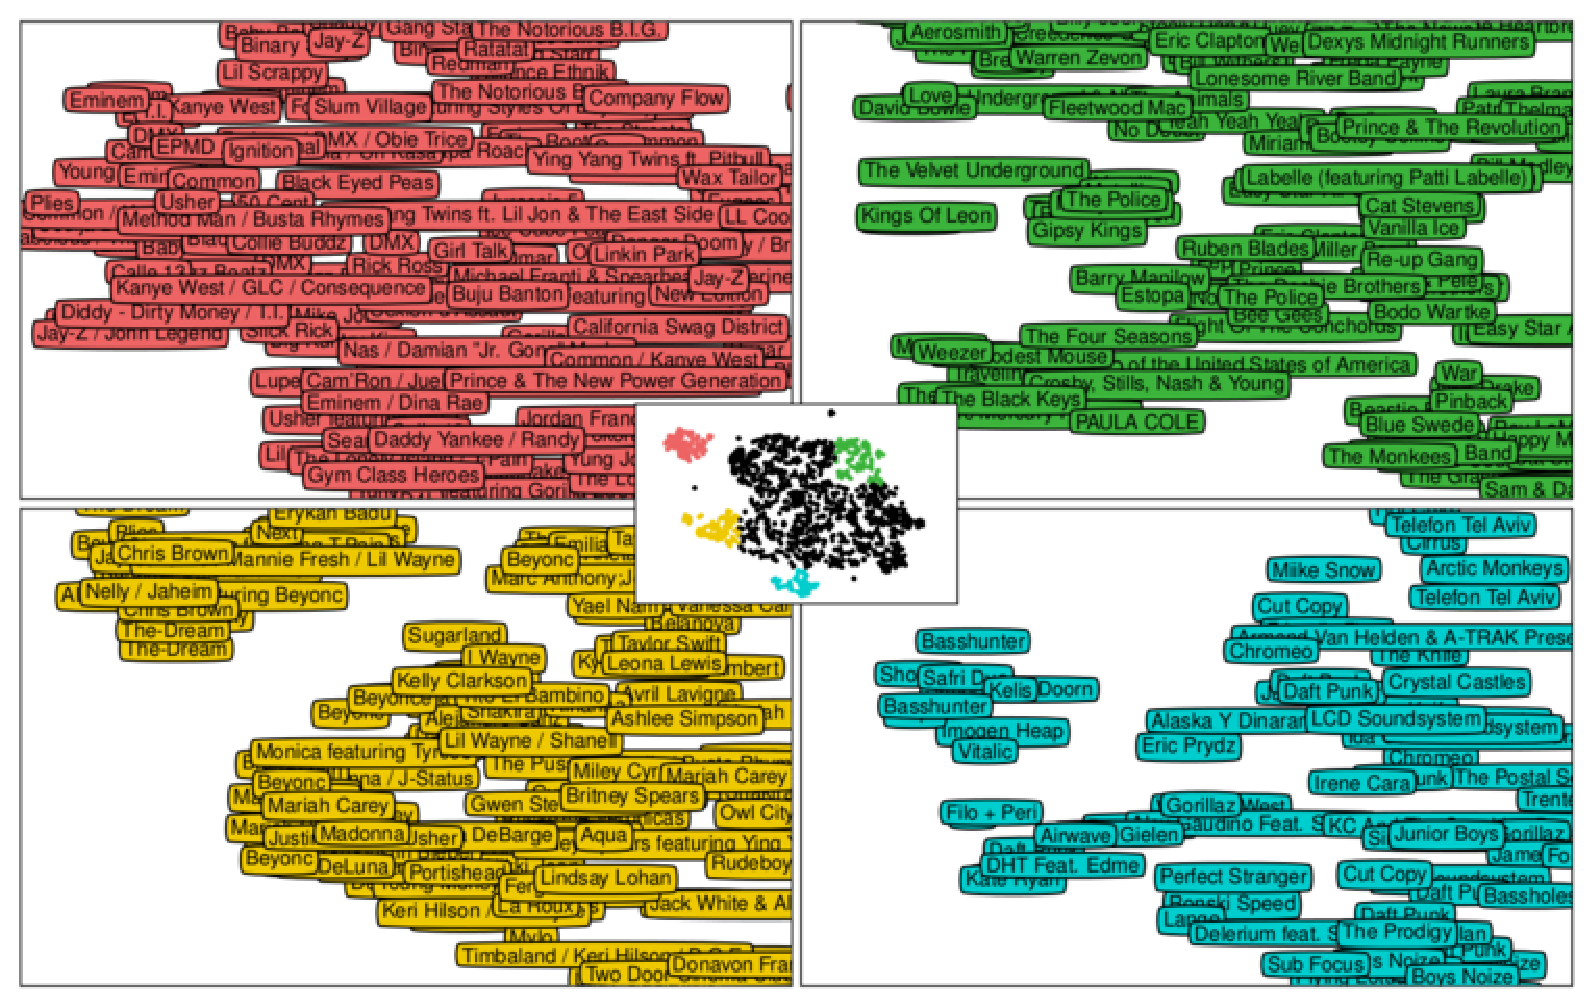
\includegraphics{clusters.eps}}}
      \caption{Visualization of the artist classification using latent factors
        predicted from audio (
        \url{http://benanne.github.io/images/prentje\_nips.png})}
      \end{figure}
    \end{center}
    \hspace*{1cm}

  \end{textblock}

  %---------------------------------------------------------------------------%
  %                                Second column.                             %
  %---------------------------------------------------------------------------%
  \begin{textblock}{7}(8,2.4)
    \Head{Dataset}
    \sf
    In order to train the CNN, we are using the MagnaTagATune dataset, which
    was made available by the Magnatune label for the research community. The
    data was collected using the TagATune game where users annotated audio
    tracks with audio relevant tags.
    \\ \\
    The dataset consists of approximately 26,000 of 29 seconds music clips
    encoded in 16 kHz, 32kbps, mono mp3, generously contributed by John
    Buckman, the founder of every MIR researcher's favorite label Magnatune.
    Each of them is annotated with a combination of 188 tags such as "orchestral",
    "orchestra", "punk", "slow", "blues", "rock" etc. It also contains music
    similarity annotations in the form of triples where given a triple of songs
    (A, B, C), metrics of how many players have flagged the song A, B or C as
    most different from the others.

    \bigskip
    \hrule
  \end{textblock}

  \begin{textblock}{7}(8,5.1)
    \Head{Architecture}
    \sf

    \Subhead{Overview}

    Our system needs to be able to suggest songs similar to that provided by
    the user, based only on its audio sample.

    To achieve this goal we first build a ground truth model using 
    MagnaTagATune dataset. Each song in the database is annotated by users with
    multiple tags that we treat as "bag of words" meaning only the presence and
    count of a tag matters and but its position. We will run word2vec algorithm
    using gensim Python toolkit on this dataset to produce latent vecotr
    representation of each song.

    We will then build a Convolutional Neural Network taking frequency spectrum
    of an audio sample as input and outputing latent vector representation. The
    Network will be trained to minimize the MSE of the predictions with the
    ground truth model.

	\bigskip

    \Subhead{Details}

    We will use compressed mel-spectograms of the audio samples to form
    compressed time-frequency representations and use them to train our CNN.
    The samples will overlap in time. We will experiment with the depth and
    size of the network. Figure 2 shows possible configuration with three
    convolutional layers and three fully connected layers.

    \begin{center}
      \begin{figure}
        \rotatebox{0}{\scalebox{1}{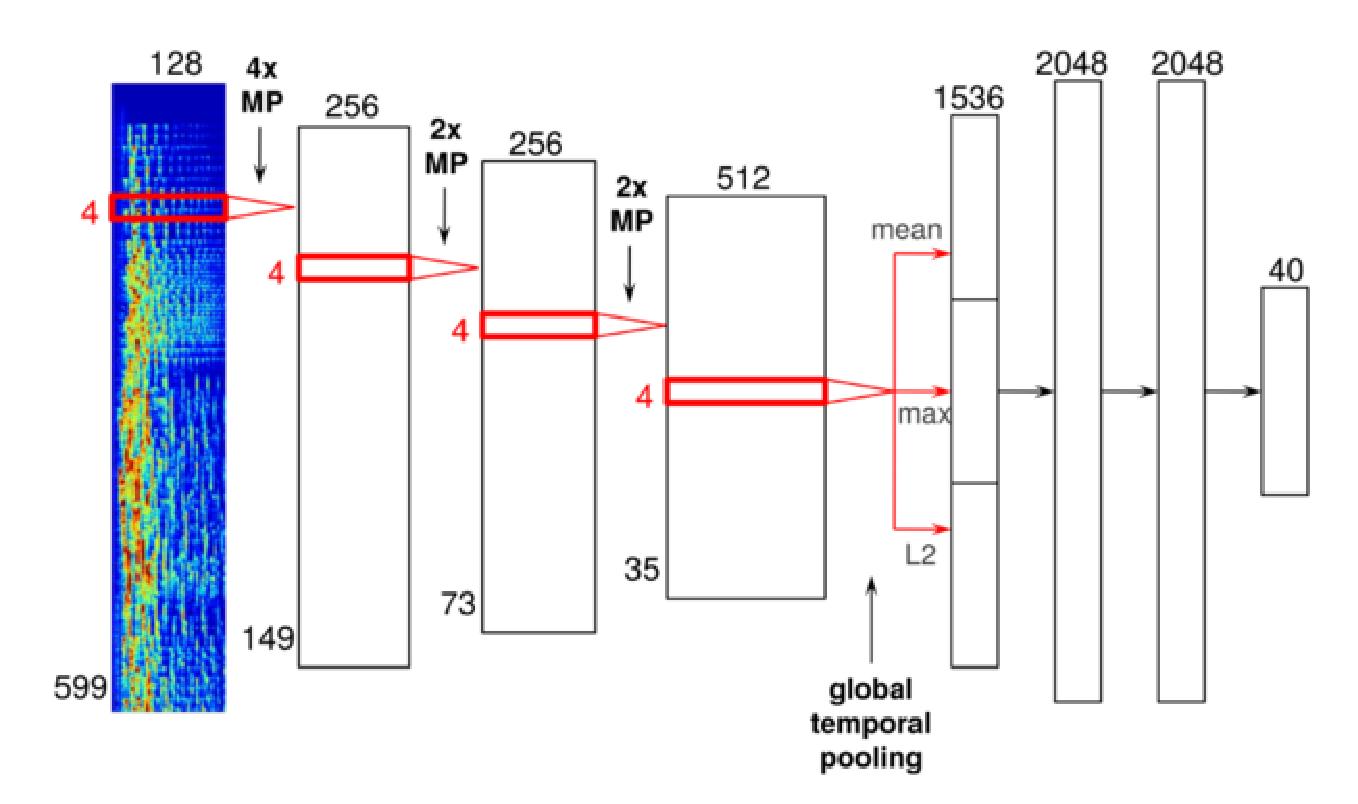
\includegraphics{cnn.eps}}}
        \caption{
          \url{http://benanne.github.io/images/spotify\_convnet.png}}
      \end{figure}
    \end{center}

    \bigskip

  \end{textblock}

  %----------------------------------------------------------------------%
  %           Third column.                                              %
  %----------------------------------------------------------------------%
  \begin{textblock}{7}(16,2.4)

    \Head{Possible Extensions}
    \sf

    \Subhead{User feedback}

    One of the possible extensions we could investigate is using user feedback
    provided through a simple interface in order to enhance the recommendation
    results. For example, there might be cases where the next proposed track
    does not satisfy the user's preferences. Having a way to collect such
    feedback could help the system fine tune music similarity data based on
    triples, including the previous, the current and the next proposed tracks.
    Though, as Dieleman references on his post, this type of feedback tends to
    be very noisy, thus we are not certain whether or not such a feature will
    improve our results.
    
    \bigskip

    \Subhead{Million Song Dataset (MSD)}

    The Million Song Dataset is a freely-available collection of audio features
    and metadata for a million contemporary popular music tracks. This is
    rather big in contrast to MagnaTagATune. Depending on the evaluation
    results, this dataset might prove useful to establish a more intelligent
    model where a greater variety of filters are learnt. However, in the
    interest of time, processing such a huge dataset in a traditional fashion
    is not an option. If necessary, using Amazon's Web services such as EMR
    (MapReduce, Spark) to process the MSD is definitely a solution.

    \bigskip
    \hrule
  \end{textblock}

  \begin{textblock}{7}(16,6.85)

  	\Head{Discussion and Conclusions}
	\sf

	Being able to classify music in the latent vector space without having usage
	data, can help companies in the industry of digital music distribution take
	more sophisticated decisions for new audio content. Having Dieleman's
	prototype description will help us make comparisons based on the evaluation
	results of both systems, for example concerning the granularity of the
	filters learnt. We expect the problem to be challenging enough, especially
	when it comes on adjusting the overlapping samples in various time frame
	sizes and deciding on the exact CNN layer architecture, for example how
	many fully connected layers does our model need.
  
	%\vspace*{4mm} % Sometimes you will have to fudge the final spacing.
	\bigskip
	\hrule
  \end{textblock}

  \begin{textblock}{7}(16,9.25)

  \Head{References}
  \sf

  [1] Deep content-based music recommendation, Aäron van den Oord, Sander
    Dieleman and Benjamin Schrauwen, NIPS 2013.

  
  \bigskip

  \end{textblock}

  %----------------------------------------------------------------------%
  %            Construction lines                                        %

  %\begin{textblock}{23}(0,2)\rule{\textwidth}{0.1mm}\end{textblock}
  % Shows where the bottom of the header bar should fall.

  %\begin{textblock}{23}(0,2.4)\rule{\textwidth}{0.1mm}\end{textblock}
  % Shows where the top of each column should start.

  %\begin{textblock}{23}(0,12)\rule{\textwidth}{0.1mm}\end{textblock}
  % Shows where the bottom of the lowest block in each column should end

  %\begin{textblock}{1.5}(6,4.12)\rule{\textwidth}{0.1mm}\end{textblock}
  %\begin{textblock}{1.5}(6,4.52)\rule{\textwidth}{0.1mm}\end{textblock}
  % Used to find the base of the first block and thus the top of the second.

  %\begin{textblock}{1.5}(14,4.85)\rule{\textwidth}{0.1mm}\end{textblock}
  %\begin{textblock}{1.5}(14,5.25)\rule{\textwidth}{0.1mm}\end{textblock}
  % Same purpose but in the second column.

  %\begin{textblock}{1.5}(15,6.05)\rule{\textwidth}{0.1mm}\end{textblock}
  %\begin{textblock}{1.5}(15,6.45)\rule{\textwidth}{0.1mm}\end{textblock}
  % Same purpose but in the third column.

%import bibliography TODO: this doesnt work
\cite{*}
\bibliography{references}{}
\bibliographystyle{plain}
\end{document}
